\documentclass[a4paper,10pt]{article}
%\usepackage[latin1]{inputenc}
\usepackage{amsfonts}
\usepackage{amssymb}
\usepackage{amsthm}
\usepackage{amsmath}
\usepackage{caption}
\usepackage{booktabs}
\usepackage[bahasai]{babel}
\usepackage[hidelinks]{hyperref}
%\usepackage[labelsep=period,format=hang,font=small]{caption}
\usepackage{caption}
\usepackage{fontenc}
\usepackage{graphicx}
\usepackage{lipsum}
\usepackage{abstract}
\usepackage{times}
\usepackage{indentfirst}
\usepackage{url}
\usepackage{titlesec}
\usepackage{multicol}
\usepackage{multirow}
\usepackage{titling}
\usepackage{tabularx}
\usepackage{microtype}
\usepackage{pgfplots}
\usepackage{tikz}
\usepackage{subfig}
\usepackage{enumitem}
\usepackage{rotating}
\usepackage{makecell}
\usepackage{colortbl}
\setlength{\droptitle}{-1.5cm}
\urlstyle{rm}
\renewcommand{\baselinestretch}{1}

\setlength{\footskip}{40pt}

\usepackage[top=19mm,bottom=43mm,left=14.32mm,right=14.32mm]{geometry}
\setlength{\tabcolsep}{4.22mm}
\renewcommand\thesection{\Roman{section}}
\renewcommand\thesubsection{\Alph{subsection}}
\renewcommand\thesubsubsection{\arabic{subsubsection})}
\renewcommand\thetable{\Roman{table}}
%\newcommand{\SSS}{\renewcommand{\baselinestretch}{1.5}\tiny \normalsize }
%\newcommand{\SDS}{\renewcommand{\baselinestretch}{1}\tiny \normalsize }

\titleformat{\section}[block]{\normalsize\filcenter\scshape\Roman{section}.}{}{0.5em}{}
\titleformat{name=\section,numberless}[block]{\normalsize\filcenter\scshape}{}{0em}{}
\titleformat{\subsection}[block]{\normalsize\itshape\Alph{subsection}.}{}{0.5em}{}
\titleformat{\subsubsection}[runin]{\normalsize\itshape}{\thesubsubsection}{0.5em}{}[:]
\titlespacing{\section}{0em}{0.25em}{0.5em}
\titlespacing{\subsection}{0em}{0.25em}{0.5em}
\titlespacing{\subsubsection}{1em}{0.25em}{0.5em}
\newenvironment{body}{\begin{multicols}{2}}{\end{multicols}}
\setlength{\parskip}{0mm}

\addto\captionsbahasai{
	\renewcommand{\abstractname}{Intisari}
	\renewcommand{\bibname}{Referensi}
	\renewcommand{\refname}{Referensi}
	\renewcommand{\tablename}{\scshape{TABEL}}
}

\let\oldthebibliography\thebibliography
\let\endoldthebibliography\endthebibliography
\renewenvironment{thebibliography}[1]{
	\begin{oldthebibliography}{#1}
		\setlength{\itemsep}{0em}
		\setlength{\parskip}{0em}
	}
	{
	\end{oldthebibliography}
}

\captionsetup[table]{format=plain,labelsep=newline,font=footnotesize,textfont=sc,justification=centering}
\captionsetup[figure]{labelsep=period,format=hang,font=footnotesize,justification=justified}

\makeatletter
\renewenvironment{table}
{\def\@captype{table}%
	\captionsetup{format=plain,labelsep=newline,font=footnotesize,textfont=sc,justification=centering}%
	\fontsize{8}{8}\selectfont
}
{}

\renewenvironment{figure}
{\def\@captype{figure}%
	\captionsetup{labelsep=period,format=hang,font=footnotesize,justification=justified}
}
{}

\makeatother

\newcommand*\annotatedFigureBoxCustom[8]{\draw[#5,thick,rounded corners] (#1) rectangle (#2);\node at (#4) [fill=#6,thick,shape=circle,draw=#7,inner sep=2pt,font=\sffamily,text=#8] {\textbf{#3}};}
%\annotatedFigureBox{bottom-left}{top-right}{label}{label-position}
\newcommand*\annotatedFigureBox[4]{\annotatedFigureBoxCustom{#1}{#2}{#3}{#4}{white}{white}{black}{black}}
\newcommand*\annotatedFigureText[4]{\node[draw=none, anchor=south west, text=#2, inner sep=0, text width=#3\linewidth,font=\sffamily] at (#1){#4};}
\newenvironment {annotatedFigure}[1]{\begin{tikzpicture}
	\node[anchor=south west,inner sep=0] (image) at (0,0) { #1};\begin{scope}[x={(image.south east)},y={(image.north west)}]}{\end{scope}\end{tikzpicture}}

\usetikzlibrary{shapes.geometric, arrows, positioning,datavisualization,patterns,decorations.markings,calc,intersections}
\tikzstyle{startstop} = [rectangle, rounded corners, minimum width=3cm, minimum height=1cm,text centered, draw=black]
\tikzstyle{io} = [trapezium, trapezium left angle=70, trapezium right angle=110, minimum width=3cm, minimum height=1cm, text centered, draw=black]
\tikzstyle{process} = [rectangle, minimum width=3cm, text width=5.5cm, minimum height=1cm, text centered, draw=black]
\tikzstyle{decision} = [diamond, minimum width=3cm, minimum height=1cm, text centered, draw=black]
\tikzstyle{arrow} = [thick,->,>=stealth]

%\renewenvironment{abstract}
%{\list{}{%
%	}%
%	\item[\noindent\textbf{\abstractname ---}]\relax}
%{\endlist}

\title{\fontsize{24}{28}\selectfont Perancangan Kontroler Lingkungan Termal \textit{Climate Chamber} Berbasis Jaringan Saraf Tiruan}
\author{\fontsize{11}{11}\selectfont Ridhan Fadhilah$^1$, Faridah$^2$, Agus Arif$^3$}
\date{}

\begin{document}
	\setlength{\abovedisplayskip}{1pt}
	\setlength{\belowdisplayskip}{1pt}	
	
	\maketitle
	
	\vspace{-1.5cm}
	
	{\centering
		{\itshape\fontsize{10}{10}\selectfont
			$^{1,2,3}$Departemen Teknik Nuklir dan Teknik Fisika FT UGM\\
			Jln. Grafika 2 Yogyakarta 55281 INDONESIA\\
		}
		{\fontsize{9}{9}\normalfont\selectfont
			$^1$ridhan.fadhilah@mail.ugm.ac.id\\
			$^2$faridah@ugm.ac.id\\
			$^3$agusarif@ugm.ac.id\\
		}
	}
	
	\vspace{0.3cm}
	
	{\setlength{\parindent}{0cm}\bfseries
		Intisari--- Penelitian-penelitan kenyamanan termal membutuhkan kondisi lingkungan termal pada \textit{Climate Chamber} (sebagai ruang uji termal) untuk dapat dikondisikan secara otomatis sesuai dengan skema pengujian penelitian. Dengan menggunakan data dari Simulasi IES-VE\cite{skripsiIchfan} dan model \textit{plant}\cite{skripsiTanto} pada penelitian sebelumnya, dalam penelitian ini dibangun kontroler berbasis jaringan saraf tiruan (JST) untuk mengendalikan suhu ruang (\textit{Tdb}) dan kelembapan relatif (\textit{RH}) pada \textit{Climate Chamber}. Kontroler dibangun dari model JST dengan menggunakan prinsip model invers dari model \textit{plant} berdasarkan data simulasi IES-VE.
		
		Kontroler JST dibangun dengan menggunakan MATLAB dan disimulasikan dengan menggunakan Simulink. JST Kontroler dibangun dengan pembagian data 80\% data latih, 10\% data validasi, dan 10\% data uji. JST Kontroler menggunakan fungsi aktivasi \textit{hyperbolic tangent} dengan algoritma pembelajaran Levenberg-Marquardt. JST Kontroler memiliki arsitektur jaringan dengan 1 lapisan tersembunyi (\textit{hidden layer}) berisi 35 neuron. Hasil perancangan mampu mengendalikan lingkungan termal \textit{Climate Chamber} dengan nilai \textit{steady-state error} sebesar 0,18$^\circ$C untuk suhu ruang dan sebesar 0,04\% untuk kelembapan relatif.\\
		
		Kata kunci--- Lingkungan Termal, Kontroler, Jaringan Saraf Tiruan, Ruang Iklim.
	}
	
	\vspace{0.3cm}
	
	{\setlength{\parindent}{0cm}\bfseries
		Abstract--- Thermal comfort studies require the thermal environment conditions in the Climate Chamber (as a thermal test room) to be automatically conditioned according to the research test scheme. By using data from the IES-VE simulation\cite{skripsiIchfan} and plant model\cite{skripsiTanto} in the previous research, this research designed a controller based on Artificial Neural Network (ANN) to control air temperature (Tdb) and relative humidity (RH) in the Climate Chamber. The Controller is designed from ANN model using the principle of plant inverse model based on IES-VE simulation data.
		
		The ANN Controller was built using MATLAB and simulated using Simulink. ANN Controller was created by split the data into 80\% training data, 10\% validation data, and 10\% testing data. ANN controller uses the hyperbolic tangent activation function with the Levenberg-Marquardt learning algorithm. ANN Controller has a network architecture with one hidden layer containing 35 neurons. The results of the author's design able to control the thermal environment of the Climate Chamber with a steady-state error value 0.18$^\circ$C for room temperature and 0.04\% for relative humidity.\\
		
		Keywords--- Thermal Environment, Controller, Artificial Neural Network, Climate Chamber.
	}
	
	\begin{body}
		\section{Pendahuluan}
		\subsection{Latar Belakang Masalah}
		Indonesia merupakan pengguna energi terbesar di Asia Tenggara antara tahun 2000 dan 2015, yaitu lebih dari 36\% penggunaan energi primer Asia Tenggara. Antara tahun 2000 dan 2015, produk domestik bruto (PDB) Indonesia bertambah dua kali lipat dan kebutuhan listrik meningkat 150\%. Pertumbuhan ekonomi mendorong peningkatan kebutuhan energi Indonesia. Pengguna energi terbesar Indonesia tahun 2015 adalah sektor rumah tangga (38\%) dan industri dan jasa (29\%), diikuti oleh transportasi (27\%) (Gambar \ref{fig:1:energy}).
		
		Efisiensi sangat penting dilakukan untuk menghemat energi. Penggunaan teknologi penyejuk ruangan yang lebih efisien diperkirakan mampu
		menghemat tagihan pelanggan listrik USD 690 juta per tahun di tahun 2030. Kebutuhan
		penyejuk ruangan tumbuh cepat dan diperkirakan bertambah dua kali lipat antara tahun
		2016 dan 2020 \cite{IEA}.
		
		\begin{figure}
			\centering
			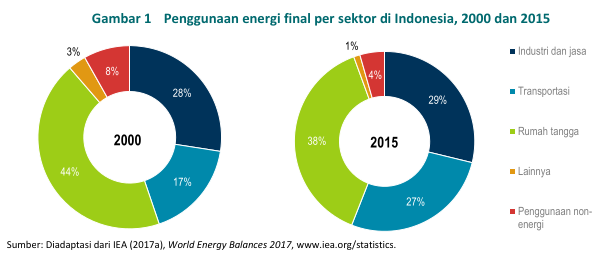
\includegraphics[width=0.5\textwidth]{figures/EnergyUsage}
			\caption{Penggunaan energi final per sektor di Indonesia, 2000 dan 2015 \cite{IEA}}
			\label{fig:1:energy}
		\end{figure}
		
		
		Ruangan pada setiap bangunan umumnya menggunakan penyejuk ruangan atau \textit{Air Conditioner} (AC) untuk mencapai kondisi yang nyaman bagi penghuni di dalamnya. Padahal hal tersebut belum tentu tepat. Sesungguhnya, penghuni tidak menginginkan kondisi ruang yang lebih dingin ataupun lebih panas dari keadaan awalnya. Penghuni ruang menginginkan kondisi ruangan yang nyaman bagi tubuh mereka. Kondisi ini yang disebut sebagai kenyamanan termal. Kenyamanan termal yang dimaksud tidaklah sesederhana upaya untuk menurunkan suhu di suatu ruangan. Kenyaman termal bergantung juga kepada sensasi termal tubuh manusia. Dengan demikian, kebutuhan energi dalam pemenuhan kenyamaan termal tersebut dapat dikatakan cukup tinggi.
		
		Kenyamanan termal didefinisikan sebagai kondisi pikiran yang mengekspresikan kepuasan terhadap lingkungan termal \cite{ASHRAE55}. Lingkungan Termal adalah lingkungan yang mempengaruhi manusia dalam hal kualitas termalnya, sehingga manusia dapat merasakan lingkungan tersebut sebagai lingkungan yang dingin atau panas. Kenyamanan termal penting untuk kesehatan dan kebugaran tubuh manusia. Hal tersebut berpengaruh terhadap produktivitas manusia dalam melakukan kegiatan. Kurangnya kenyamanan termal dapat mengakibatkan kondisi stres bagi penghuni bangunan. Apabila kondisi bangunan terlalu panas, maka penghuni akan merasa lelah. Apabila kondisi bangunan terlalu dingin, maka penghuni akan merasa gelisah dan bimbang. Karena terdapat variasi yang besar, baik secara fisiologis maupun psikologis, dari orang ke orang, sulit untuk memuaskan semua orang di suatu ruang. Kondisi lingkungan yang dibutuhkan untuk kenyamanan tidak sama untuk semua orang. 
		
		Kenyamanan termal secara fisiologis bergantung kepada proses perpindahan kalor antara tubuh dan lingkungan dimana respon fisiologis tubuh berupaya untuk mempertahankan suhu inti tubuh agar tetap bernilai konstan. Untuk mempelajari respon fisiologis tersebut, dibutuhkan sebuah \textit{climate chamber} dimana kondisi iklim di dalamnya dapat dikendalikan sesuai dengan kebutuhan penelitian.\\
		
		\subsection{Tujuan Penelitian}
		Penelitian ini bertujuan untuk membangun model kontroler berbasis jaringan saraf tiruan dengan meninjau nilai \textit{steady-state error} untuk mengendalikan lingkungan termal pada \textit{climate chamber} DTNTF FT-UGM.\\
		
		\subsection{Batasan Masalah}\label{batasan masalah}
		\begin{enumerate}
			\item Model \textit{plant} menggunakan model berbasis jaringan saraf tiruan yang dibuat oleh Tri Hartanto\cite{skripsiTanto}.
			\item Kinerja kontroler hanya ditinjau melalui nilai \textit{steady-state error} karena secara fisis respon transien termal pada bangunan berlangsung cukup lama.
			\item Perancangan kontroler dilakukan pada aplikasi MATLAB karena memiliki fitur JST dan dianggap mudah untuk menjalankan simulasi sistem kendali pada SIMULINK.
		\end{enumerate}
		
		\section{Metodologi Penelitian}
		\subsection{Alat dan Bahan}
		Alat dan bahan disajikan pada Tabel \ref{tbl:4:alatbahan} dan Tabel \ref{tbl:4:speklaptop}.
		
		\begin{table}
			\centering
			\caption{Daftar alat dan bahan}
			\label{tbl:4:alatbahan}
			\fontsize{8}{8}\selectfont
			\begin{tabularx}{\linewidth}{clX}\toprule
				No. & Nama alat/bahan & Fungsi \\
				\toprule
				1 & ASUS N550JX & Perangkat komputer \\ \midrule
				2 & \textit{Climate Chamber} & Objek penelitian \\ \midrule
				3 & IES-VE 2019 & Perangkat lunak untuk pengambilan data lingkungan termal \textit{climate chamber} dan variasi gangguan \\ \midrule
				4 & MS Excel 365 & Perangkat lunak pengolahan data tabular \\ \midrule
				5 & MATLAB R2018a & Perangkat lunak pemrograman dalam merancang jaringan saraf tiruan untuk kontroler. \\ \midrule
				6 & SIMULINK & Perangkat lunak untuk mewujudkan simulasi sistem kontrol. \\ \bottomrule
			\end{tabularx}
		\end{table}
		
		\begin{table}
			\centering
			\caption{Spesifikasi laptop ASUS N550JX}
			\label{tbl:4:speklaptop}
			\fontsize{8}{8}\selectfont
			\begin{tabularx}{\linewidth}{clX}\toprule
				No. & Komponen & Spesifikasi \\ \toprule
				1 & \textit{Processor} & Intel Core i7-4720HQ CPU @ 2.60GHz x 8 \\ \midrule
				2 & \textit{Graphics} & Intel Haswell Mobile \\ \midrule
				3 & RAM & 8 GB \\ \midrule
				4 & Tipe sistem operasi & 64-bit \\ \midrule
				5 & Sistem operasi & Windows 10 Home Single Language \\ \bottomrule
			\end{tabularx}
		\end{table}
		
		\subsection{Penentuan Tuntutan Rancangan}
		
		Tuntutan rancangan Tugas Akhir ini yaitu kontroler mampu mengendalikan \textit{plant} dengan skenario penggunaan \textit{climate chamber}, yaitu menggunakan \textit{set point} ramp (16$^{\circ}$C-30$^{\circ}$C) dengan lompatan 2$^{\circ}$C.
		
		\subsection{Pengambilan Data Simulasi IES-VE}\label{subsec:lang_bench}
		Penelitian ini menggunakan data yang sama dengan data yang digunakan oleh penelitian Tri Hartanto\cite{skripsiTanto} yang bersumber dari model yang telah dibuat pada penelitian sebelumnya berjudul "Karakterisasi Lingkungan Termal Chamber Iklim Menggunakan Metode Simulasi CFD dengan Perangkat Lunak IES-VE" yang diteliti oleh Ichfan Kurniawan \cite{skripsiIchfan}.  Data tersebut merupakan hasil simulasi pada \textit{software} IES-VE dengan menerapkan beberapa variasi kondisi lingkungan pada model \textit{climate chamber}. Variasi tersebut yaitu kondisi batas lingkungan (radiasi matahari dan suhu bola kering luar / \textit{outdoor dry bulb temperature}), kondisi AC, dan kondisi \textit{heater}. Variasi kondisi batas lingkungan tersebut diwujudkan dalam pembagian 4 musim dalam 1 tahun, yakni bulan Maret, Juni, September dan Desember. Keluaran dari model IES-VE berupa nilai suhu ruang (\textit{air temperature}) \textit{chamber} dan kelembapan relatif (RH) \textit{chamber}. Dari model tersebut didapatkan nilai MAE perhitungan selisih variabel lingkungan termal hasil simulasi dan pengukuran lapangan sebesar 0,8 $\pm$ 0,7$^{\circ}$C untuk suhu udara ruang dan 2,5 $\pm$ 3,8\% untuk kelembaban relatif \cite{skripsiIchfan}. Data yang sudah terkumpul disajikan dalam bentuk data tabular.
		
		\subsubsection{Kondisi \textit{Climate Chamber}}
		
		Climate chamber memiliki ukuran panjang $\times$ lebar $\times$ tinggi = 3 m $\times$ 2 m $\times$ 3 m. Komponen-komponen di dalam \textit{climate chamber} terdiri dari meja, kursi, \textit{blower}, penghuni, lampu, \textit{heater}, dan AC. Posisi setiap komponen di dalam \textit{climate chamber} digambarakan pada Gambar \ref{fig:4:KondisiChamber}.\\
		
		\begin{figure}
			\centering
			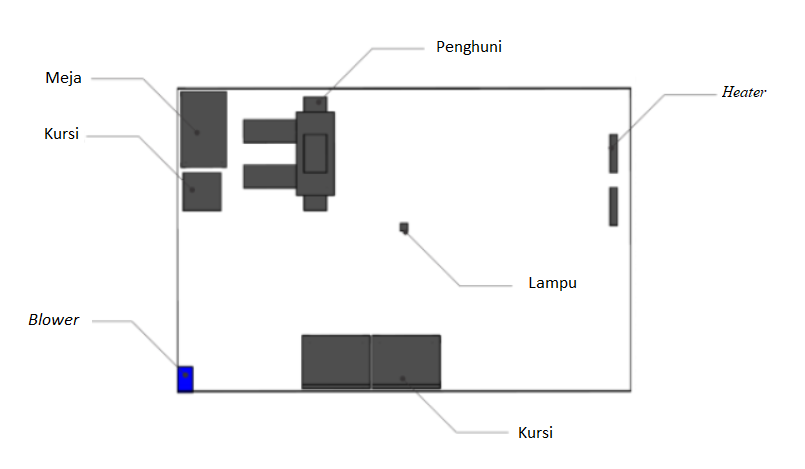
\includegraphics[width=0.5\textwidth]{figures/KondisiChamber}
			\caption{Posisi Komponen-Komponen di dalam \textit{Climate Chamber}}
			\label{fig:4:KondisiChamber}
		\end{figure}
		\vspace{1em}
		
		\begin{figure}
			\centering
			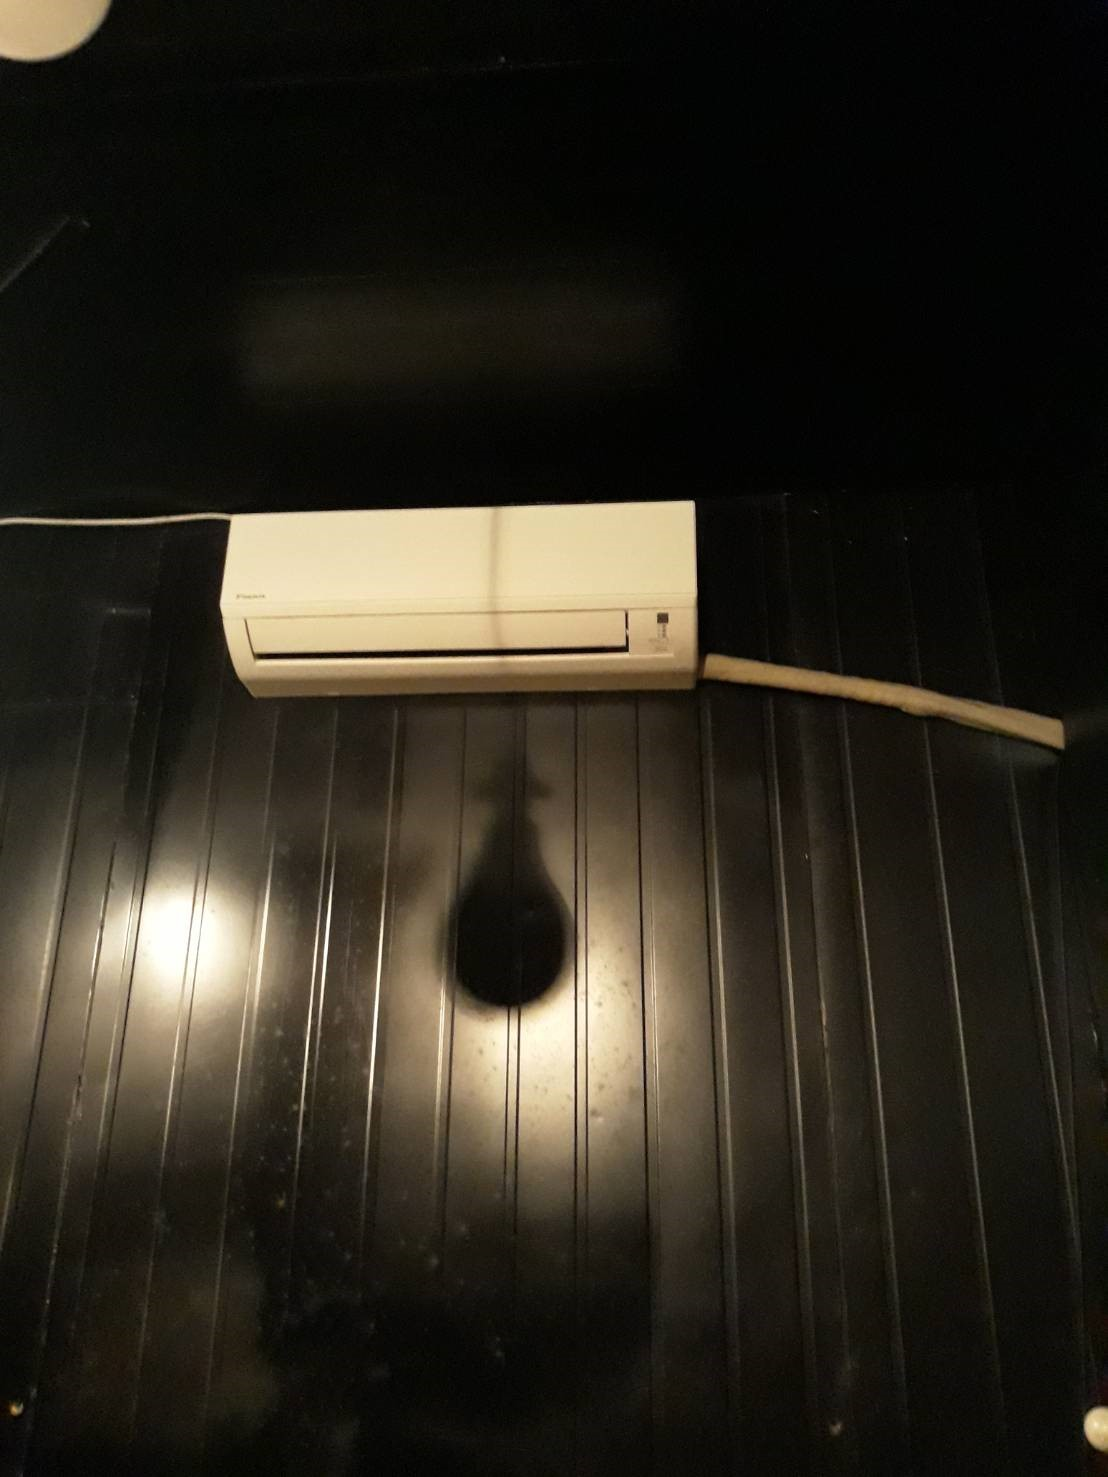
\includegraphics[width=0.3\textwidth]{figures/AC}
			\caption{Perangkat AC}
			\label{fig:4:AC}
		\end{figure}
		\vspace{1em}
		
		Perangkat AC yang berada di dalam \textit{Climate Chamber} DTNTF FT-UGM memiliki daya sebesar 2800W (1 PK). Perangkat AC mampu mengkondisikan lingkungan melalui aliran udara yang keluar. Oleh karena itu, Perangkat AC sangatlah berpengaruh terhadap kondisi lingkungan termal di dalam ruangan. Penampakan wujud perangkat AC dapat dilihat pada Gambar \ref{fig:4:AC}
		
		\begin{figure}
			\centering
			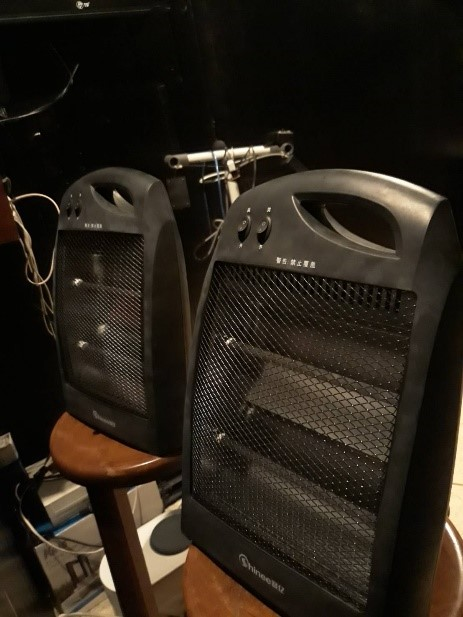
\includegraphics[width=0.15\textwidth]{figures/Heater}
			\caption{Perangkat Heater}
			\label{fig:4:Heater}
		\end{figure}
		\vspace{1em}
		
		Perangkat pemanas (\textit{heater}) yang berada di dalam \textit{climate chamber} memiliki daya sebesar 900W. Terdapat dua buah perangkat pemanas di dalam \textit{climate chamber}. Semakin banyak perangkat pemanas yang aktif maka suhu ruang akan menjadi semakin meningkat. Kenaikan rerata suhu ruang yaitu sebesar $\pm1,9^\circ$C untuk setiap perangkat pemanas. Penampakan wujud \textit{heater} dapat dilihat pada Gambar \ref{fig:4:Heater}.
		
		Selain faktor di dalam \textit{climate chamber}, faktor dari luar ruangan pun secara tidak langsung mempengaruhi kondisi lingkungan termal \textit{climate chamber}, di antaranya adalah suhu lingkungan (\textit{dry bulb temperature}) dan intensitas radiasi matahari. Posisi harian matahari mempengaruhi perubahan nilai suhu lingkungan dan intensitas radiasi matahari. Pada siang hari (posisi \textit{altitude} matahari ketika berada tepat di atas \textit{climate chamber}) memberikan paparan radiasi matahari yang mengenai selubung bangunan. Hal ini menyebabkan kenaikan suhu di dalam \textit{climate chamber}.
		
		\subsubsection{Rancangan Skenario Pengambilan Data}
		Rancangan skenario pada \textit{climate chamber} menghasilkan kombinasi antara perangkat AC dan jumlah \textit{heater} dalam kondisi ON. Peangkat AC dikondisikan untuk menyala dari pukul 08:00 sampai dengan pukul 17:00 WIB bervariasi dengan rentang nilai 16$^\circ$C - 30$^\circ$C dengan lompatan 1$^\circ$C. Jumlah \textit{heater} dalam kondisi ON terbagi menjadi 3 kondisi, yaitu keduanya tidak menyala (berkode 0), salah satu menyala (berkode 1), dan keduanya menyala (berkode 2). Kombinasi tersebut menghasilkan 25 variasi skenario.
		
		Untuk variasi suhu lingkungan dan intensitas radiasi matahari digunakan 4 titik ekstrim bumi terhadap matahari yaitu pada tanggal 21 Maret, 21 Juni, 23 September dan 22 Desember. Kemudian dilakukan simulasi pada setiap titik tersebut dengan kombinasi pada Gambar \ref{fig:4:SkenarioData}. Dengan demikian, total skenario yang dihasilkan dari kombinasi tersebut berjumlah 100 skenario.
		
		\begin{figure}
			\centering
			
\includegraphics[width=0.3\textwidth]{figures/SkenarioData}
			\caption{Skenario Pengambilan Data}
			\label{fig:4:SkenarioData}
		\end{figure}
		\vspace{1em}
		
		\subsubsection{Simulasi IES-VE}
		
		Pada Gambar \ref{fig:4:HasilSimulasiIESVE} ditunjukkan salah satu hasil simulasi untuk skenario AC 26$^\circ$C dan \textit{heater} ON 2 buah dengan variabel gangguan yang digambarkan pada Gambar \ref{fig:4:LoadSimulasiIESVE}. Grafik yang ditampilkan terdiri dari 4 parameter yaitu suhu lingkungan (\textit{To}), intensitas radiasi matahari (RD), suhu ruang (\textit{Tdb}), dan kelembapan relatif (RH). Skenario ini dilakukan selama 24 jam dengan selang waktu pengambilan data selama 6 menit dimulai dari pukul 00:03 hingga 23:57 WIB. Selang waktu tersebut adalah waktu tersingkat yang dapat dilakukan pada software IES-VE 2019. Respon waktu suhu ruang terhadap aktivasi AC tidak diperhitungkan dikarenakan secara fisis, respons transien termal pada bangunan berlangsung cukup lama, sehingga hanya berfokus untuk meninjau nilai kesalahan keadaan-ajeg (\textit{steady-state error}).\\
		
		\begin{figure}
			\centering
			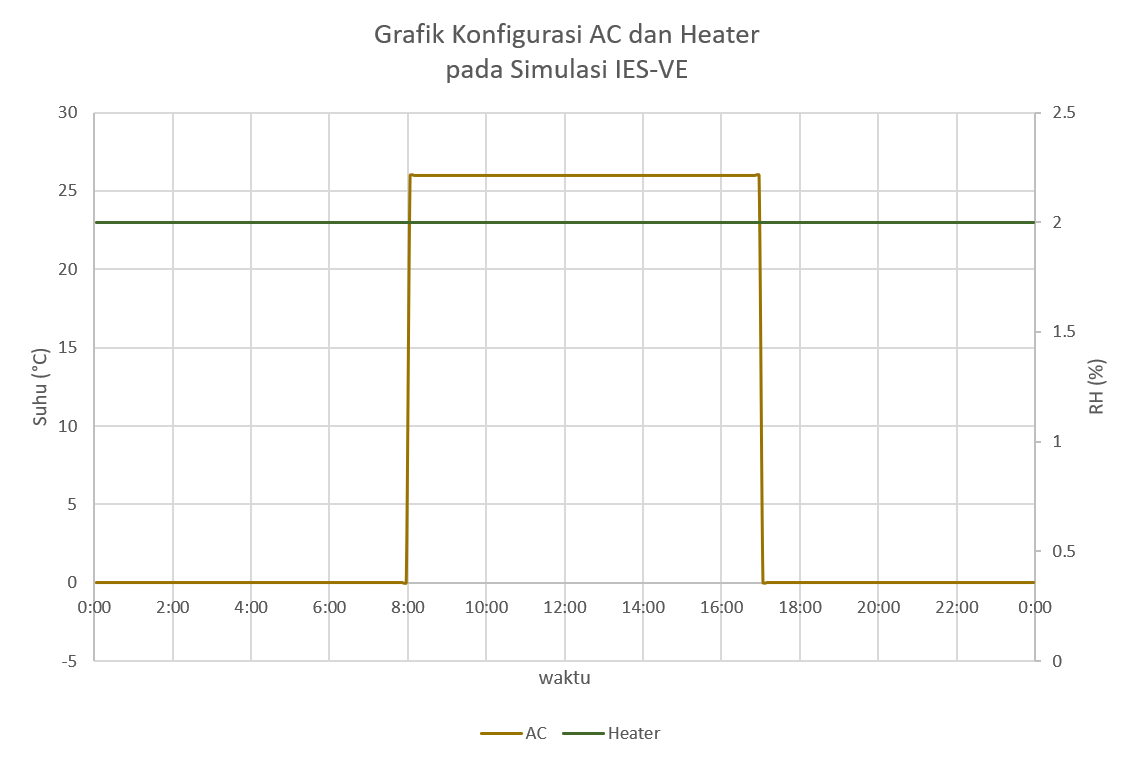
\includegraphics[width=0.4\textwidth]{figures/ACHTSimulasiIESVE}
			\caption{Data Konfigurasi AC dan \textit{Heater} pada Simulasi ISE-VE}
			\label{fig:4:ACHTSimulasiIESVE}
		\end{figure}
		
		\begin{figure}
			\centering
			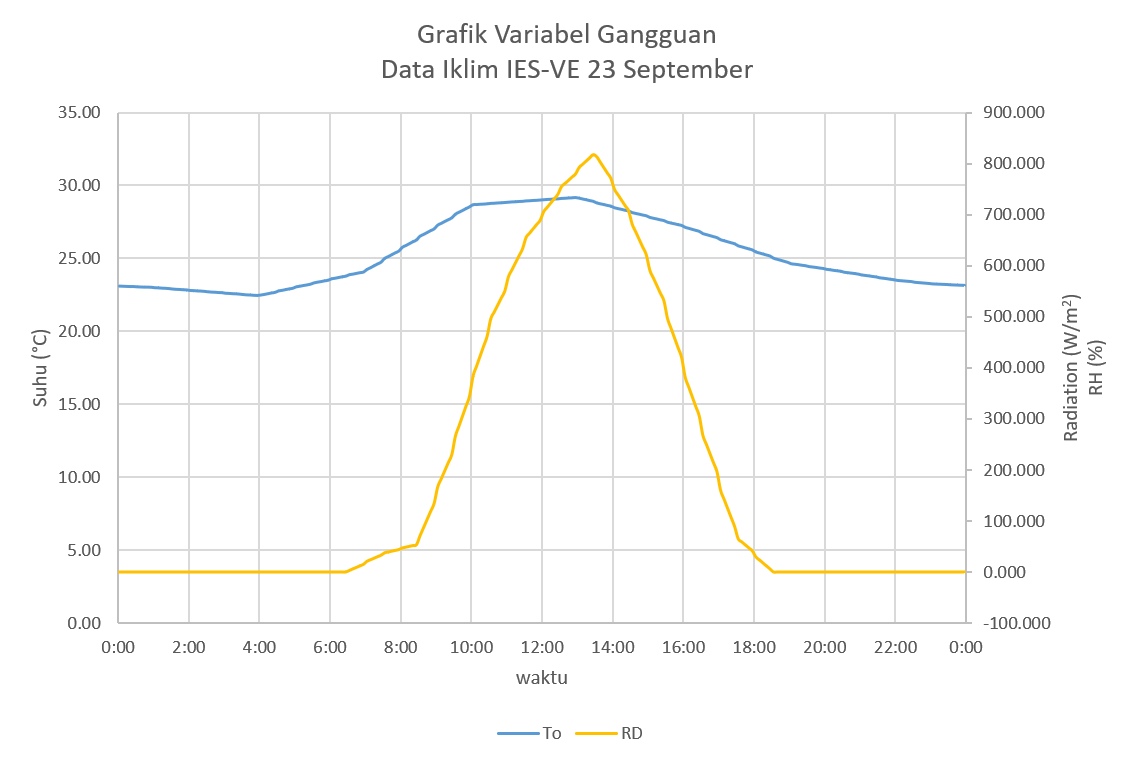
\includegraphics[width=0.4\textwidth]{figures/LoadSimulasiIESVE}
			\caption{Variabel Gangguan Simulasi ISE-VE}
			\label{fig:4:LoadSimulasiIESVE}
		\end{figure}
		
		\begin{figure}
			\centering
			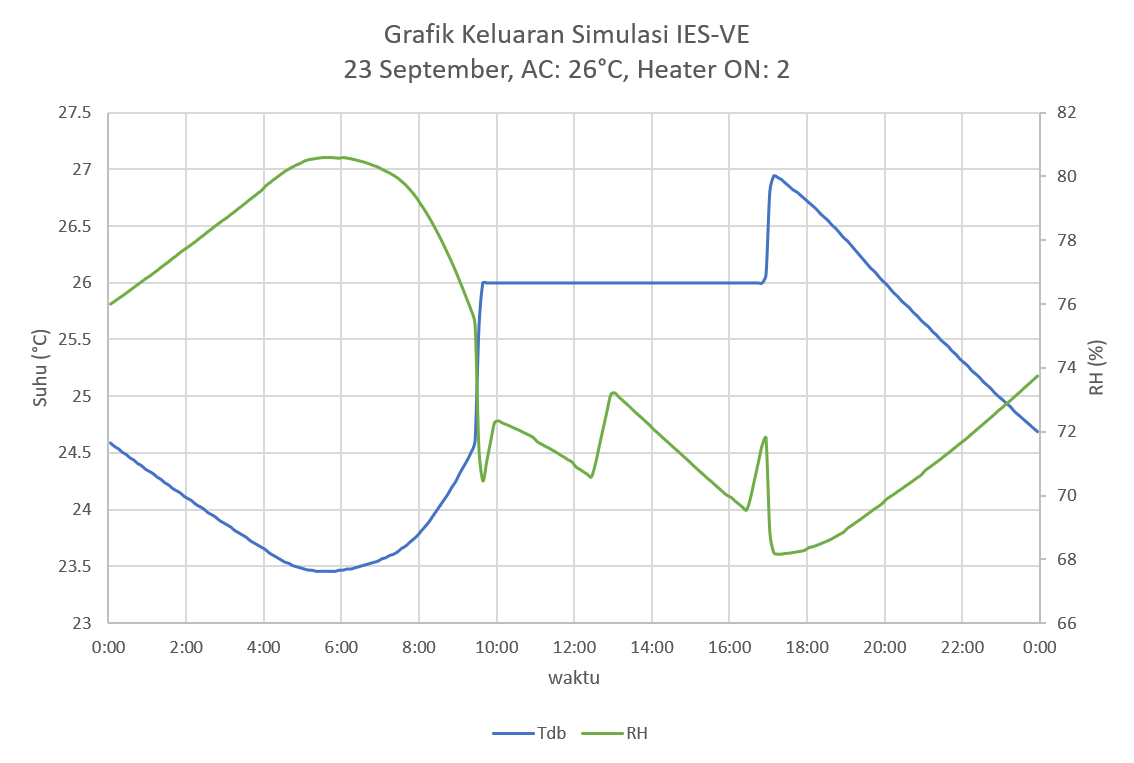
\includegraphics[width=0.4\textwidth]{figures/HasilSimulasiIESVE}
			\caption{Data Hasil Simulasi ISE-VE}
			\label{fig:4:HasilSimulasiIESVE}
		\end{figure}
		\vspace{1em}
		
		\subsection{Model JST Plant}\label{subsec:4:err}
		
		Model \textit{plant} pada penelitian ini menggunakan model plant JST yang telah dirancang pada penelitian sebelumnya\cite{skripsiTanto}. Model plant tersebut memiliki nilai MAE perhitungan antara target dan prediksi sebesar 0,59$^{\circ}$C untuk suhu ruang dan 5,44\% untuk kelembapan relatif. Akurasi JST sebesar 96,23\% untuk suhu ruang dan 68,90\% untuk kelembapan relatif. Arsitektur Model Plant JST digambarkan pada Gambar \ref{fig:4:NNPlantModelDesign}.\\
		
		\begin{figure}
			\centering
			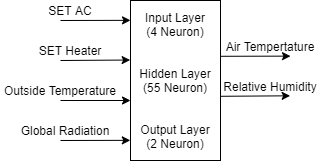
\includegraphics[width=0.3\textwidth]{figures/NNPlantModelDesign}
			\caption{Arsitektur Model Plant JST}
			\label{fig:4:NNPlantModelDesign}
		\end{figure}
		
		\subsection{Perancangan Kontroler JST}
		
		Dalam melakukan pemodelan kontrol, pertama-tama didefinisikan terlebih dahulu pasangan data masukan dan keluaran dari sistem kendali. Nilai pasangan masukan dan keluaran kontrol ditunjukkan dengan Gambar \ref{fig:4:NNControlIO}. Pasangan masukan dan keluaran tersebut didapatkan dengan memperhatikan diagram blok sistem pengendalian. Diagram blok sistem pengendalian ditunjukkan pada Gambar \ref{fig:4:ConstrolSystemBlockDiagram}.\\
		
		\begin{figure}
			\centering
			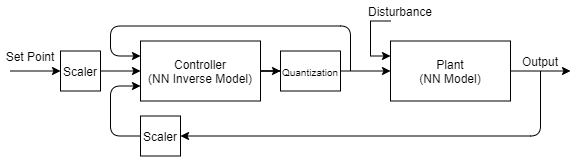
\includegraphics[width=0.5\textwidth]{figures/ControlDesignDiagramII}
			\caption{Diagram blok sistem kontrol berbasis JST\cite{paper42Paisan}}
			\label{fig:4:ConstrolSystemBlockDiagram}
		\end{figure}
	\vspace{1em}
		
		\begin{figure}
			\centering
			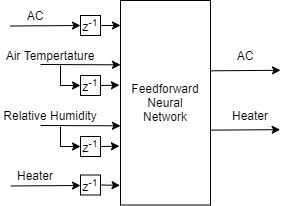
\includegraphics[width=0.25\textwidth]{figures/NNControllerIO}
			\caption{Pasangan masukan dan keluaran model JST kontroler}
			\label{fig:4:NNControlIO}
		\end{figure}
	
		Kontroler dibangun dari model JST dengan menggunakan prinsip model invers dari model \textit{plant}. Perancangan JST untuk kontroler menggunakan delay umpan balik AC, delay umpan balik \textit{heater}, output \textit{plant} dan delay output \textit{plant} sebagai sebagai masukan untuk pelatihan JST. Kemudian, pasangan data AC dan \textit{heater} digunakan sebagai pasangan data keluaran (data target) untuk pelatihan JST. Arsitektur JST kontroler dibangun dengan menggunakan \textit{feedforward neural network} atau biasa disebut juga sebagai \textit{multilayer perceptron} (MLP). Model JST akan dilatih menggunakan data hasil simulai IES-VE yang telah digunakan pula dalam pemodelan \textit{plant} oleh Tri Hartanto\cite{skripsiTanto}. Pada proses pelatihan JST, dilakukan penskalaan terhadap semua input JST menggunakan metode \textit{Min Max Scaling} kecuali variabel delay umpan masuk AC dan \textit{heater}. Penskalaan bertujuan untuk meningkatkan kinerja JST menjadi optimal dengan menyamakan rentang nilai dan besar satuan dari setiap variabel (berupa rentang nilai dari 0 hingga 1).\\
		
		\section{Hasil dan Pembahasan}
		\subsection{Identifikasi Sistem}
		
		Dalam perancangan sistem kendali, perlu diidentifikasi terlebih dahulu variabel-variabel yang terlibat pada suatu sistem. Terdapat beberapa variabel yang terlibat pada sistem \textit{climate chamber}. Variabel-variabel yang diangkat pada penelitian ini tunjukkan oleh diagram blok \textit{plant} pada Gambar \ref{fig:5:DiagramBlokPlant}. Berdasarkan diagram tersebut, dapat dikatakan bahwa sistem merupakan sistem MIMO (\textit{Multi Input Multi Output}) yaitu sistem yang memiliki beberapa masukan dan beberapa keluaran. Identifikasi sistem yang telah dilakukan akan menghasilkan suatu diagram blok fungsional sistem ditunjukkan pada Gambar \ref{fig:5:DiagramBlokSistem}.\\
		
		\begin{figure}
			\centering
			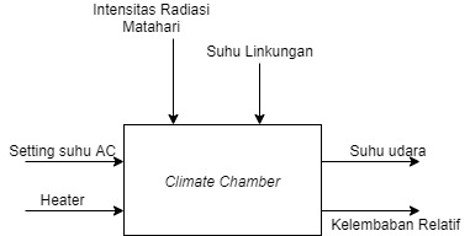
\includegraphics[width=0.35\textwidth]{figures/BlokDiagramPlant}
			\caption{Diagram Blok \textit{Plant}}
			\label{fig:5:DiagramBlokPlant}
		\end{figure}
		\vspace{1em}
		
		Dalam sistem \textit{climate chamber}, variabel manipulasi yang digunakan adalah \textit{setting} suhu AC dan \textit{heater} (jumlah \textit{heater} ON). Kemudian, variabel kontrol yang digunakan yaitu suhu udara (Tdb) dan kelembapan relatif (RH) pada \textit{plant} / \textit{climate chamber}. Ada pula variabel gangguan sistem yaitu berupa intensitas radiasi matahari dan suhu lingkungan. Untuk pengujian \textit{set point}, skenario pengujian mengadaptasi Tugas Akhir pengujian level sensasi termal yang dilakukan oleh Nur Muna\cite{skripsiMuna}. Hanya saja pada penelitian menggunakan \textit{set point} step bertingkat dengan lompatan 2$^{\circ}$C dari nilai suhu sebesar 16$^{\circ}$C hingga 30$^{\circ}$C.\\
		
		\begin{figure}
			\centering
			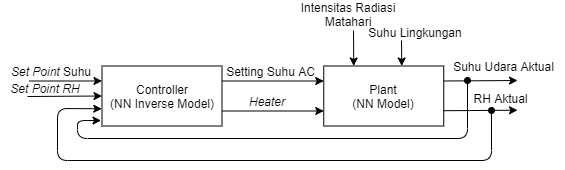
\includegraphics[width=0.5\textwidth]{figures/DiagramBlokFungsionalSistem}
			\caption{Diagram Blok Fungsional Sistem}
			\label{fig:5:DiagramBlokSistem}
		\end{figure}
		
		Kontroler pada \textit{climate chamber} memiliki enam buah variabel masukan dan dua buah variabel keluaran. Variabel masukan kendali ini yaitu nilai \textit{set point} suhu udara, \textit{set point} kelembapan relatif, nilai aktual umpan balik suhu udara, nilai aktual umpan balik kelembapan relatif, nilai umpan balik \textit{setting} suhu AC, dan nilai umpan balik \textit{heater}. Sementara, variabel keluaran kontroler ini adalah \textit{setting} suhu AC dan \textit{heater} (jumlah \textit{heater} ON).
		
		Untuk memaksimalkan kinerja kontroler, pada proses pelatihan JST (kontroler) dilakukan pengskalaan terhadap semua variabel masukan JST menggunakan metode \textit{Min Max Scaling} kecuali variabel umpan balik \textit{setting} suhu AC dan variabel umpan balik \textit{heater}. Pengskalaan bertujuan untuk meningkatkan kinerja JST menjadi optimal dengan menyamakan rentang nilai dan besar satuan dari setiap variabel (berupa rentang nilai dari 0 hingga 1). Masing-masing variabel diubah menjadi skala satuan dengan melakukan transformasi data secara statistik. Data dari setiap variabel akan dikurangi dengan nilai minimum variabel tersebut yang dikemudian dibagi oleh selisih dari nilai maksimum dan nilai minimum variabel tersebut. Dengan demikian, ditambahkan pula blok \textit{scaler} pada diagram blok sistem kontrol agar nilai masukan kontroler dapat disesuaikan.
		
		\begin{figure}
			\centering
			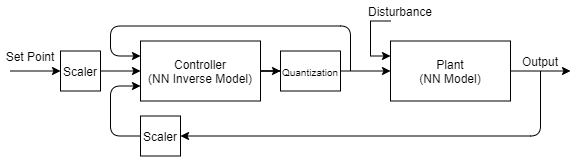
\includegraphics[width=0.5\textwidth]{figures/ControlDesignDiagramII}
			\caption{Diagram blok sistem kontrol berbasis JST}
			\label{fig:5:ConstrolSystemBlockDiagram}
		\end{figure}
		
		Diagram blok sistem kontrol juga memiliki blok tambahan berupa blok kuantisasi (\textit{Quantization}). Blok ini berperan sebagai penyesuai nilai variabel manipulasi yang dihasilkan kontroler. Hal ini dilakukan karena pada praktiknya nilai \textit{setting} suhu AC merupakan nilai bilangan bulat dan bukan nilai bilangan desimal. Hal ini pun berlaku untuk variabel manipulasi \textit{heater} dimana nilainya berupa nilai 0, 1, atau 2 yang menunjukkan jumlah \textit{heater} ON / menyala. Sehingga tidak mungkin ada nilai diantara nilai tersebut. Dengan demikian, diagram blok dipasangi sebuah blok kuantisasi (\textit{Quantization}) yang berfungsi untuk menghindari nilai desimal atau pun nilai yang berada di luar rentang nilai variabel manipulasi. Pada akhirnya dihasilkan diagram blok sistem kontrol yang ditunjukkan pada Gambar \ref{fig:5:ConstrolSystemBlockDiagram}.\\
		
		\subsection{Model Plant JST}
		
		Model \textit{plant} pada penelitian ini menggunakan model JST yang telah dibangun oleh Tri Hartanto\cite{skripsiTanto}. Arsitektur model dirancang dengan memperhatikan sistem \textit{plant} pada Gambar \ref{fig:5:DiagramBlokPlant}. Arsitektur memiliki nilai-nilai \textit{hyperparameter} yang dirangkum pada Tabel \ref{tbl:5:NNPlantTanto}.
		
		\begin{table}
			\caption{Tabel Rancangan Model Plant JST\cite{skripsiTanto}}
			\label{tbl:5:NNPlantTanto}
			\centering
			% use packages: array
			\begin{tabularx}{\linewidth}{ll}\toprule
				\textbf{Nama Hyperparameter} & \textbf{Nilai Hyperparameter} \\ \toprule
				Arsitektur & Feedforward Neural Network \\ \midrule
				Pembagian Data & 50\% 25\% 25\% \\ \midrule 
				Jumlah Layar Tersembunyi & 1 \\ \midrule
				Jumlah Neuron pada Layar & [55] \\ \midrule
				Fungsi Aktivasi Layar & Hyperbolic Tangent \\ \midrule
				Algoritma Pembelajaran & Levenberg-Marquardt \\ \midrule
				Mean Absolute Error (MAE) & Tdb: 0,59$^\circ$C ; RH: 5,44\% \\ \midrule
				Mean Squared Error (MSE) & Tdb: 0,75$^\circ$C ; RH: 52,33\% \\ \midrule
				Koefisien Korelasi (R) & Tdb: 96,23\% ; RH: 68,90\% \\ \bottomrule
			\end{tabularx}
		\end{table}
		
		\subsection{Rancangan Kontroler JST}
		\subsubsection{Variasi Pembagiaan Data}
		
		Variasi pembagiaan data dilakukan dengan membandingkan beberapa variasi pembagiaan data ke dalam 5 variasi. Kemudian kinerja dari setiap pembagian data dibandingkan dengan konfigurasi hyperparameter pada Tabel \ref{tbl:5:NeuronVariation}.
		
		\begin{table}
			\centering
			\caption{Tabel Daftar Variasi Pembagian Data}
			\label{tbl:5:NeuronVariation}
			\begin{tabularx}{\linewidth}{XX}\toprule
				\textbf{Pembagian Data} & \textbf{Persentase Data} \\ \toprule
				Pembagian Data 1 & (50\% 25\% 25\%) \\ \midrule
				Pembagian Data 2 & (60\% 20\% 20\%) \\ \midrule
				Pembagian Data 3 & (70\% 15\% 15\%) \\ \midrule
				Pembagian Data 4 & (80\% 10\% 10\%) \\ \midrule
				Pembagian Data 5 & (80\% 15\% 05\%) \\ \bottomrule
			\end{tabularx}
		\end{table}
		\vspace{1em}
		
		Model JST untuk membandingkan variasi pembagian data menggunakan arsitektur \textit{feedforward network} dengan 1 lapisan tersembunyi berisi 10 neuron. Pada tabel yang disajikan, pembagian data ditulis dengan format ’Pembagian Data n’ dan ’(x\% y\% z\%)’ dimana n = nomor variasi, x = pembagian data pelatihan, y = pembagian data validasi, dan z = pembagian data pengujian. Berdasarkan hasil variasi yang ditunjukkan pada Gambar \ref{fig:5:DataSplittingVariation}, didapatkan pembagian data terbaik yaitu pembagian data bernama "Pembagian Data 4". Data dibagi menjadi 3 bagian, yakni 80\% data pelatihan, 10\% data validasi, dan 10\% data pengujian.\\
		
		\begin{figure}
			\centering
			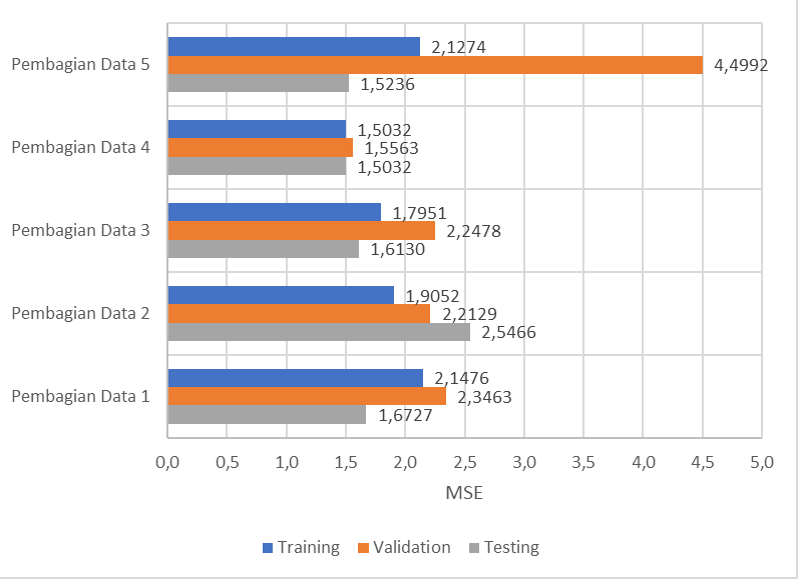
\includegraphics[width=0.5\textwidth]{figures/VariasiPembagianDataJSTKontroler}
			\caption{Grafik Variasi Pembagian Data}
			\label{fig:5:DataSplittingVariation}
		\end{figure}
		
		\subsubsection{Variasi Arsitektur JST Kontroler}
		Pada perancangan model JST kontroler digunakan 2 variasi fungsi aktivasi, yaitu fungsi tansig (fungsi \textit{hyperbolic tanget}) dan fungsi logsig (fungsi sigmoid). Kemudian masing-masing dilatih dengan jumlah neuron yang bervariasi dari 5 neuron hingga 60 neuron dengan lompatan sebesar 5 neuron. Dari proses variasi ini, didapatkan hasil bahwa model yang menggunakan fungsi aktivasi tansig dengan 35 neuron menghasilkan kinerja dengan nilai MSE terkecil. Hasil dari variasi ini ditunjukkan pada Gambar \ref{fig:5:ActivationVariation}.
		
		\begin{figure}
			\centering
			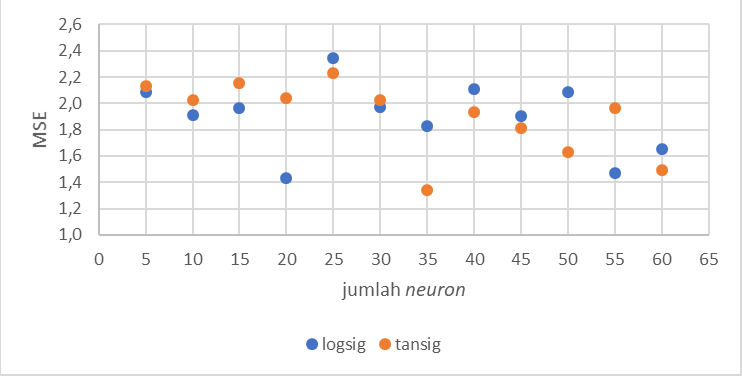
\includegraphics[width=0.5\textwidth]{figures/ActivationVariation}
			\caption{Grafik Persebaran MSE Variasi Arsitektur JST Kontroler}
			\label{fig:5:ActivationVariation}
		\end{figure}
		
		\begin{figure}
			\centering
			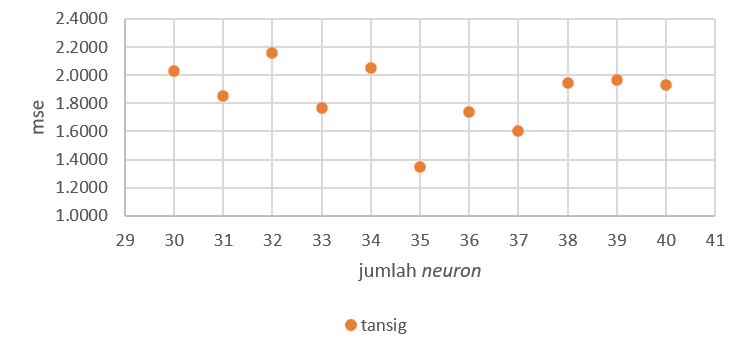
\includegraphics[width=0.5\textwidth]{figures/NeuronVariation}
			\caption{Grafik Persebaran MSE Variasi Arsitektur JST Kontroler}
			\label{fig:5:NeuronVariation}
		\end{figure}
		\vspace{1em}
		
		Kemudian arsitektur JST divariasikan kembali menggunakan fungsi aktivasi tansig dari 30 neuron hingga 40 neuron dengan lompatan sebesar 1 neuron untuk mengetahui kinerja model pada jumlah neuron yang berdekatan. Setelah dilakukan variasi, didapatkan hasil bahwa model JST dengan 35 neuron masih merupakan model arsitektur terbaik dengan nilai MSE terkecil. Hasil variasi ini dapat dilihat pada Gambar \ref{fig:5:NeuronVariation}.
		
		\subsubsection{Hasil Rancangan Model JST Kontroler}
		Setelah dilakukan perancangan model JST melalui variasi arsitektur model, didapatkan rancangan model JST kontroler terbaik. Model JST dibangun dengan arsitektur \textit{feedforward neural network} 1 lapisan tersembunyi dengan 35 neuron. Model JST menggunakan fungsi aktivasi tansig (\textit{hyperbolic tanget}) dan algoritma pembelajaran Levenberg-Marquardt. Model JST Kontroler terbaik memiliki nilai \textit{hyperparameter} yang diringkas pada Tabel \ref{tbl:5:NNControl}.
		
		\begin{table}
			\centering
			\caption{Tabel Rancangan Kontroler JST (\textit{NN Inverse Model})}
			\label{tbl:5:NNControl}
			% use packages: array
			\begin{tabularx}{\linewidth}{XX}\toprule
				\textbf{Nama Hyperparameter} & \textbf{Nilai Hyperparameter} \\ \toprule
				Arsitektur & Feedforward Neural Network \\ \midrule
				Pembagian Data & 80\% 10\% 10\% \\ \midrule 
				Jumlah Layar Tersembunyi & 1 \\ \midrule
				Jumlah Neuron pada Layar & [35] \\ \midrule
				Fungsi Aktivasi Layar & Hyperbolic Tangent (tansig) \\ \midrule
				Algoritma Pembelajaran & Levenberg-Marquardt \\ \midrule
				Mean Absolute Error (MAE) & AC: 0,37$^\circ$C ; HT: 0,02\\ \midrule
				Mean Squared Error (MSE) & AC: 2,68$^\circ$C ; HT: 0,01\\ \midrule
				Koefisien Korelasi (R) & AC: 99,12\% ; HT: 99,65\% \\ \bottomrule
			\end{tabularx}
		\end{table}
				
		\subsection{Hasil Simulasi Kontrol SIMULINK}
		
		Pada simulasi kontrol, digunakan nilai \textit{set point} sesuai dengan uji eksperimental level sensasi termal yang dilakukan oleh Nur Muna pada \textit{climate chamber}\cite{skripsiMuna}. Perbedaannya, pada penelitian ini variasi naik turun suhu dari 16$^\circ$C hingga 30$^\circ$C menggunakan lompatan sebesar 2$^\circ$C.
		
		\subsubsection{Skenario Pemanasan Pendinginan dengan Variabel Gangguan Konstan}
		
		Pada simulasi ini digunakan nilai variabel gangguan konstan sebesar 26,8$^\circ$C untuk suhu lingkungan dan 423,343 $W/m^2$ untuk intensitas radiasi matahari. Nilai-nilai variabel gangguan tersebut merupakan nilai rerata dari variabel gangguan pada jam operasi penggunaan \textit{climate chamber}, yaitu pukul 08:00 WIB sampai dengan pukul 17:00 WIB. Berdasarkan hasil simulasi, kontroler mampu mengendalikan suhu ruang dan kelembapan relatif mengikuti nilai \textit{set point}. Akan tetapi, kontroler tidak mampu menaikan suhu ruang mencapai nilai lebih dari 27$^\circ$C. Hal ini dapat terjadi diakibatkan nilai manipulator AC tidak mampu melebihi nilai maksimum (SET 30$^\circ$C). Kombinasi \textit{set point} dan hasil simulasi ditunjukkan pada Gambar \ref{fig:5:SimulinkTd} untuk suhu ruang dan Gambar \ref{fig:5:SimulinkRH} untuk kelembapan relatif.
		
		Dengan meninjau nilai variabel manipulasi AC yang ditunjukkan pada Gambar \ref{fig:5:SimulinkAC}, dapat dilihat bahwa untuk mengendalikan suhu mencapai \textit{set point} 26$^\circ$C, perangkat AC perlu mengeluarkan sinyal sebesar 28$^\circ$C (waktu ke-100 hingga ke-120). Dengan demikian, ketika \textit{set point} bernilai 28$^\circ$C, perangkat AC hanya mampu mengeluarkan sinyal maksimum 30$^\circ$C (waktu ke-120 hingga ke-140).
		
		\begin{figure}
			\centering
			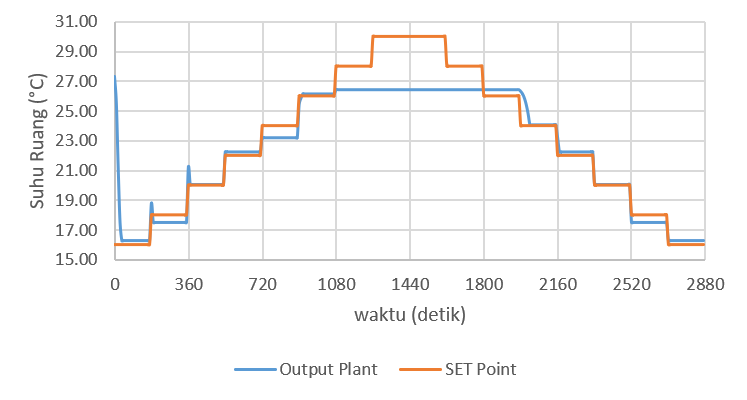
\includegraphics[width=0.5\textwidth]{figures/Simulink1Td}
			\caption{Grafik Hasil Simulasi Simulink untuk Suhu Ruang}
			\label{fig:5:SimulinkTd}
		\end{figure}
		\vspace{1em}
		
		\begin{figure}
			\centering
			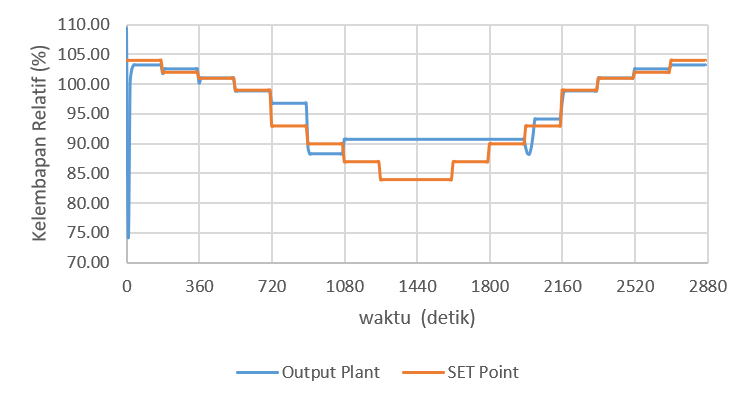
\includegraphics[width=0.5\textwidth]{figures/Simulink1RH}
			\caption{Grafik Hasil Simulasi Simulink untuk Kelembapan Relatif}
			\label{fig:5:SimulinkRH}
		\end{figure}
		\vspace{1em}
		
		\begin{figure}
			\centering
			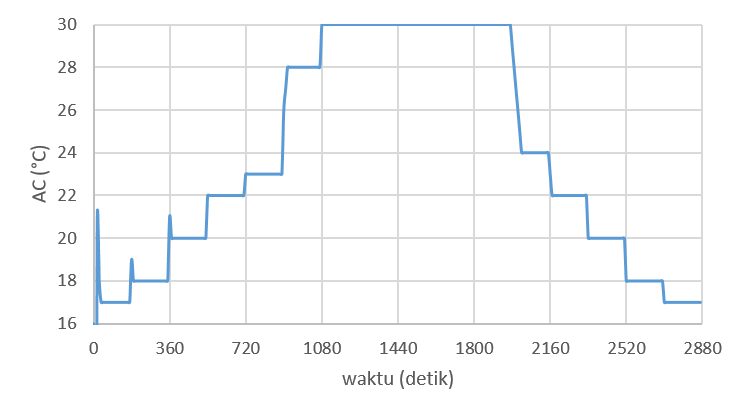
\includegraphics[width=0.5\textwidth]{figures/Simulink1AC}
			\caption{Grafik Variabel Manipulasi AC pada Simulasi Simulink}
			\label{fig:5:SimulinkAC}
		\end{figure}
		\vspace{1em}
		
		\begin{figure}
			\centering
			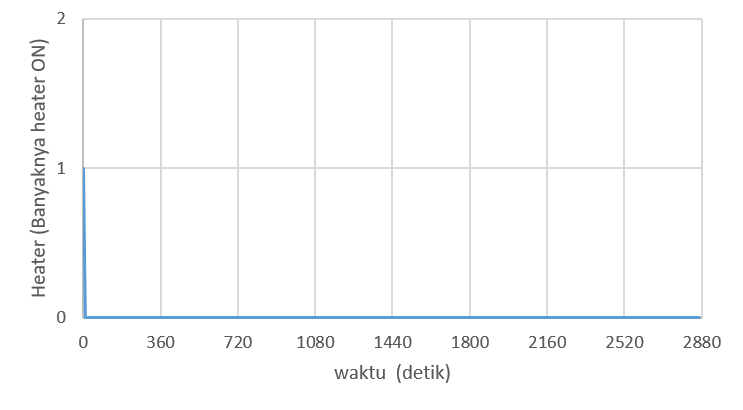
\includegraphics[width=0.5\textwidth]{figures/Simulink1HT}
			\caption{Grafik Variabel Manipulasi \textit{Heater} pada Simulasi Simulink}
			\label{fig:5:SimulinkHT}
		\end{figure}
		\vspace{1em}
		
		Kurangnya kehandalan kinerja kontroler pada penelitian ini untuk mengendalikan suhu ruang di atas \textit{set point} 26$^\circ$C disebabkan oleh salah satu kelemahan model JST dalam pemodelan \textit{plant}. Secara fisis, proses pemanasan pada sistem bangunan (dalam hal ini \textit{climate chamber}) membutuhkan waktu yang cukup lama. Dengan demikian, proses pemanasan pada kenyataannya tetap bisa mencapai \textit{set point} suhu di atas 26$^\circ$C. Hanya saja proses tersebut membutuhkan waktu (\textit{settling time}) yang cukup lama. Akan tetapi, proses tersebut tidak dapat disimulasikan secara sempurna pada penelitian ini dikarenakan model JST \textit{plant} yang dibangun oleh Tri Hartanto\cite{skripsiTanto} hanya berupa model pasangan data dan bukan berupa model yang bergantung terhadap waktu. Sehingga, model JST \textit{plant} hanya dapat langsung mengeluarkan suatu nilai keluaran setiap menerima nilai masukan.
		
		Ditinjau dari \textit{set point} 16$^\circ$C hingga 26$^\circ$C, didapatkan nilai \textit{steady-state error} untuk suhu ruang sebesar 0,15$^\circ$C pada proses pemanasan dan sebesar 0,2$^\circ$C pada proses pendinginan. Lalu, didapatkan pula nilai \textit{steady-state error} untuk kelembapan relatif sebesar 0,05\% pada proses pemanasan dan sebesar 0,02\% pada proses pendinginan. Sehingga rerata nilai \textit{steady-state error} sebesar 0,18$^\circ$C untuk suhu ruang dan sebesar 0,04\% untuk kelembapan relatif.\\
		
		\subsubsection{Skenario Pemanasan Pendinginan dengan Variabel Gangguan Bergerak}
		
		Pada skenario ini digunakan data variabel gangguan pada 21 Juni 2019 yang bergerak dari pukul 08:03 sampai dengan 08:51 WIB. Nilai dari variabel gangguan ditunjukkan pada Gambar \ref{fig:5:Simulink2To} untuk suhu lingkungan dan \ref{fig:5:Simulink2RD} untuk intensitas radiasi matahari. Pada skenario ini, nilai \textit{set point} yang digunakan senilai dengan nilai \textit{set point} pada simulasi dengan variabel gangguan konstan.
		
		\begin{figure}
			\centering
			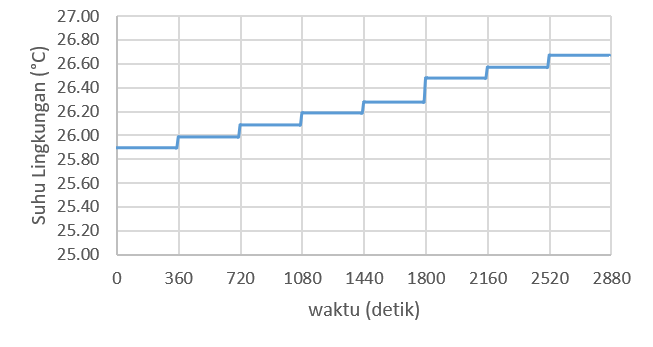
\includegraphics[width=0.5\textwidth]{figures/Simulink2To}
			\caption{Grafik Nilai Variabel Gangguan Suhu Lingkungan}
			\label{fig:5:Simulink2To}
		\end{figure}
		\vspace{1em}
		
		\begin{figure}
			\centering
			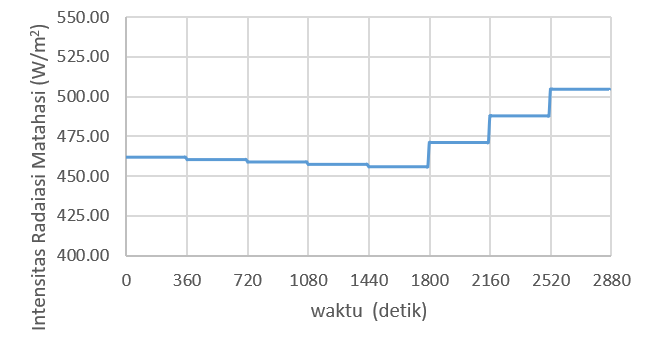
\includegraphics[width=0.5\textwidth]{figures/Simulink2RD}
			\caption{Grafik Nilai Variabel Gangguan Intensitas Radiasi Matahari}
			\label{fig:5:Simulink2RD}
		\end{figure}
		\vspace{1em}
		
		\begin{figure}
			\centering
			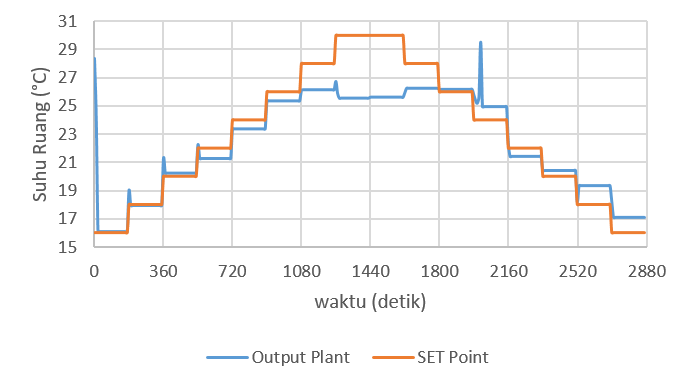
\includegraphics[width=0.5\textwidth]{figures/Simulink2Td}
			\caption{Grafik Hasil Simulasi Simulink untuk Suhu Ruang}
			\label{fig:5:Simulink2Td}
		\end{figure}
		\vspace{1em}
		
		Hasil simulasi dengan variabel gangguan bergerak pun menunjukan kinerja yang kurang optimal. Berdasarkan Gambar \ref{fig:5:Simulink2Td}, dapat dilihat bahwa kontroler tidak mampu menaikan suhu ruang mencapai nilai lebih dari 27$^\circ$C. Dapat dilihat pula bahwa terjai lonjakan nilai suhu udara pada detik ke-1980. Lonjakan tersebut terjadi akibat penonaktifan AC yang dilakukan oleh kontroler yang dapat dilihat pada Gambar \ref{fig:5:Simulink2AC}. Pada proses pendinginan, nilai \textit{steady-state error} tampak lebih besar dibandingkan saat proses pemanasan. Hal ini mungkin disebabkan karena kenaikan suhu lingkungan dan intensitas radiasi matahari. Walaupun nilai galat membesar, dapat dilihat bahwa pada proses pendinginan kontroler tetap berupaya untuk mengikuti perubahan \textit{set point}.
		
		\begin{figure}
			\centering
			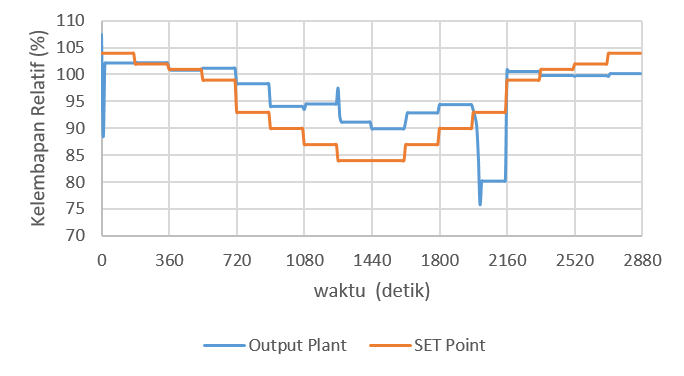
\includegraphics[width=0.5\textwidth]{figures/Simulink2RH}
			\caption{Grafik Hasil Simulasi Simulink untuk Kelembapan Relatif}
			\label{fig:5:Simulink2RH}
		\end{figure}
		\vspace{1em}
		
		\begin{figure}
			\centering
			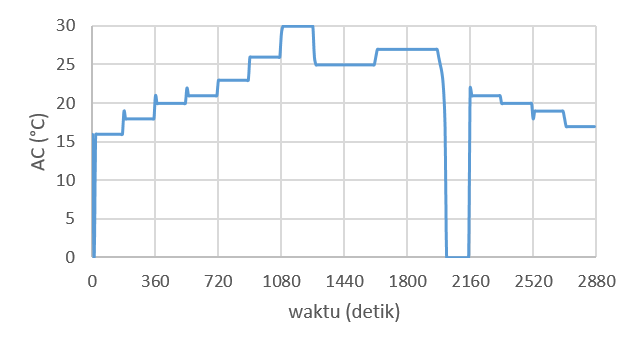
\includegraphics[width=0.5\textwidth]{figures/Simulink2AC}
			\caption{Grafik Variabel Manipulasi AC pada Simulasi Simulink}
			\label{fig:5:Simulink2AC}
		\end{figure}
		\vspace{1em}
		
		\begin{figure}
			\centering
			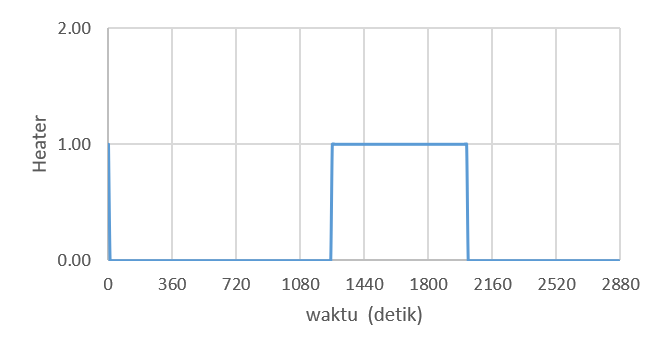
\includegraphics[width=0.5\textwidth]{figures/Simulink2HT}
			\caption{Grafik Variabel Manipulasi \textit{Heater} pada Simulasi Simulink}
			\label{fig:5:Simulink2HT}
		\end{figure}
		\vspace{1em}
		
		Dari hasil 2 simulasi yang telah dijabarkan, kontroler jarang sekali mengaktifkan 2 \textit{heater} bahkan ketika ingin mencapai suhu yang tinggi. Hal ini menimbulkan kecurigaan terhadap rentang kinerja JST, baik pada model kontroler maupun model \textit{plant}. Diketahui bahwa pada umumnya jika jumlah data pelatihan JST kurang banyak dalam men-generalisasi suatu sistem, maka kinerja dari model JST pun akan menjadi kurang optimal. Hal ini merupakan salah satu kelemahan penggunaan model JST.\\
		\vspace{3em}
		
		\section{Kesimpulan}
		Rancangan kontroler berbasis jaringan saraf tiruan memiliki nilai \textit{steady-state error} sebesar 0,18$^\circ$C untuk suhu ruang dan sebesar 0,04\% untuk kelembapan relatif. Akan tetapi, kontroler tidak mampu mengendalikan suhu ruang \textit{climate chamber} di atas nilai \textit{set point} 26$^\circ$C dikarenakan model \textit{plant}[2] bukan merupakan model yang bergantung terhadap waktu.
		
		Kontroler berbasis jaringan saraf tiruan yang dihasilkan dibangun dengan pembagian data 80\% data latih, 10\% data validasi, dan 10\% data uji. Model Kontroler JST menggunakan fungsi aktivasi \textit{hyperbolic tangent} dengan algoritma	pembelajaran Levenberg-Marquardt. Model Kontroler JST terdiri dari 1 lapisan tersembunyi dengan 35 neuron.\\
		
		\section{Saran}
		\begin{enumerate}[nolistsep]
			\item Memperkaya data pelatihan model JST menggunakan data pengukuran langsung pada \textit{climate chamber} dalam merancang kontroler JST.
			\item Menambahkan semacam manipulator/aktuator pada \textit{climate chamber} untuk memanipulasi kelembapan relatif ruang secara langsung seperti penelitian yang dilakukan oleh Jan Drgona[15]. Contoh: \textit{humidifier} dan \textit{dehumidifier}.
			\item Menambahkan variabel control lainnya ke dalam rancangan kontroler, seperti kecepatan angin, RH lingkungan, dsb.
		\end{enumerate}
		\vspace{1em}
		
		\section*{Ucapan Terima Kasih}
		Penulis mengucapkan banyak terima kasih kepada kedua pembimbing tugas akhir penulis, yaitu Faridah, S.T., M.Sc., dan Ir. Agus Arif, M.T., Tim \textit{Climate Chamber} DTNTF, serta rekan-rekan perkuliahan UGM: M. N. Fathurrahman, Irfanda Husni Sahid, M. Armand A., Tri Hartanto, Ivan Ega Pratama, dan Vandy Achmad.
		
		\bibliographystyle{skripsi}
		\bibliography{pustaka}
	\end{body}
\end{document}